\documentclass{ivoa}
\input tthdefs

\usepackage[utf8]{inputenc}
\usepackage{todonotes}
\usepackage{listings}
\usepackage{natbib}
\lstloadlanguages{XML}
\lstset{flexiblecolumns=true,basicstyle=\small,tagstyle=\ttfamily}

\SVN$Rev$
\SVN$Date$
\SVN$URL$

\hyphenation{name-space}

\newcommand{\oaiop}[1]{\textit{#1}}

\ivoagroup{Registry}


\author{Theresa Dower}
\author{Markus Demleitner}
\author{Kevin Benson}
\author{Ray Plante}
\author{Elizabeth Auden} 
\author{Matthew Graham} 
\author{Gretchen Greene} 
\author{Martin Hill}
\author{Tony Linde} 
\author{Dave Morris} 
\author{Wil O`Mullane}
\author{Guy Rixon} 
\author{Aur\'elien St\'eb\'e}
\author{Kona Andrews}

\editor{Theresa Dower}
\editor {Markus Demleitner}

\previousversion[http://www.ivoa.net/documents/RegistryInterface/20091104/]
{IVOA Registry Interfaces 1.0, IVOA Recommendation 2009-11-04}


\title{Registry Interfaces}

\begin{document}

\begin{abstract}
The VO Registry provides a mechanism with which VO applications can
discover and select resources that are relevant for a particular
scientific problem. This specification defines the operation of this
system. It is based on a general, distributed model composed of
searchable and publishing registries, as introduced at the beginning of
this document. The main body of the specification has three components:
(a) an interface for harvesting publishing registries, which builds upon
the Open Archives Initiative Protocol for Metadata Harvesting.  (b) A
VOResource extension for registering registry services and description
of a central list of said IVOA registry services.  (c) A discussion of
the Registry of Registries as the root component of data discovery in
the VO.
\end{abstract}


\section{Introduction}

\label{introduction}

In the Virtual Observatory (VO), registries provide a means for
discovering useful resources, i.e., data and services.  This discovery
takes place by searching within structured descriptions of resources,
the resource records, authored by the data providers.  In order to avoid
a single point of failure for the VO, the Registry is distributed.
This means that each data provider can run a service injecting
resource records into the Registry (a ``publishing registry'' as defined
below), and anyone can run services that allow global discovery (a
``searchable registry'' as defined below).

To enable this, common mechanisms for registry communication and
interaction are required.
This document therefore describes the standard interfaces that enable
interoperable registries.  Through these interfaces, registry
builders have a common way of sharing resource descriptions with users,
applications, and other registries.

This specification does not cover interfaces for global discovery, which
are the subject of other IVOA standards.  Also, service operators are
free to build interactive, end-user interfaces in
any way that best serves their target community.

While the architecture and standard processes for distributed registry
search and maintenance remain similar to this document's version 1.0 and
it remains backward compatible, there is a significant philosophical
change in this update. Most importantly, a defined search interface
using SOAP technology is no longer recommended, and a Table Access 
Protocol service using a registry data model is encouraged for search, with the
understanding that new technologies will continue to be developed and adopted.

\subsection{Registry Architecture and Definitions}

\label{arch}

A \emph{registry} is first a repository of structured descriptions of
resources. In the VO, a \emph{resource} is defined by the IVOA
Recommendation ``Resource Metadata for the Virtual Observatory''
\citep{std:RM}, henceforth referred to as RM, as being


\begin{quotation}
a general term referring to a VO element that can be
described in terms of who curates or maintains it and which can be
given a name and a unique identifier. Just about anything can be a
resource: it can be an abstract idea, such as sky coverage or an
instrumental setup, or it can be fairly concrete, like an organization
or a data collection.
\end{quotation}

Organizations, data collections, and services can be considered 
classes of resources. The most important type of resource to
applications is a service that actually does something. A registry
(lower case),
then, is ``a service for which the response is a structured description
of resources'' (RM).

This specification is based on the general IVOA model for registries
\citep{2004ASPC..314..585P}, which builds on RM's model
for resources.  In this model, the VO environment features
different types of registries that serve different functions. The
primary distinction is between publishing registries and searchable
ones. A secondary distinction is full versus partial.

A \emph{searchable registry} is one that allows users and client
applications to search for resource records using selection criteria
against the metadata contained in the records. The purpose of this type
of registry is to aggregate descriptions of many resources distributed
across the network. By providing a single place to locate data and
services, applications are spared from having to visit many different
sites just to determine which ones are relevant to the scientific
problem at hand. A searchable registry gathers its descriptions from
across the network through a process called \emph{harvesting}.

A \emph{publishing registry} is one that simply exposes its resource
descriptions to the VO environment in a way that allows those
descriptions to be harvested. The contents of these registries tend to
be limited to resources maintained by one or a few providers and thus
are local in nature; for example, a data center will run its own
publishing registry to allow other VO components to gather metadata on
the data center's published services.
Since the purpose is simply publishing and not to serve
users and applications directly, it is not necessary to support full
searching capabilities. This simplifies the requirements for a
publishing registry: 
storage, management, and indexing of the records can be simpler, as
there is no need to support a
search interface facilitating complex discovery queries.
While a searchable registry in practice will necessitate the
use of a database system, a simple publishing registry may get by
storing its records as flat files on disk.

Note that some registries can play both roles; that is, a searchable
registry may also publish its own resource descriptions.

A secondary distinction is full versus local. A \emph{full registry}
is one that attempts to contain records of all resources known to the VO.
Several such registries exist, run by various VO projects.  A
\emph{local registry}, on the other hand, contains only a subset of
known resources. While for publishing registries this subset usually is
defined by what services are maintained by the registry's operator,
other selection criteria are conceivable.  For instance, the IVOA's
Education IG is considering running a registry only containing resources
manually selected for suitability for primary and secondary education.

As mentioned above, harvesting is the mechanism by which a registry can
collect resource records from other registries. It is used by full
registries to aggregate resource records from publishing
registries. It can also be used to synchronize two registries to ensure
that they have the same contents. Harvesting, in this specification, is
modeled as a pull operation between two registries. The term
\emph{harvester} refers to the registry that wishes to receive records
(usually a full searchable registry); it sends its request to the
\emph{harvestee} (usually a publishing registry), which responds with
the records.  Harvesting is a much simpler process than a fully-featured
search interface, as only very few constraints need to be supported and
only full records are being transmitted in responses.  
Consequently, different protocols are  employed for the
two types of registry operations.

In this text, ``registry'' in lower case refers to concrete services,
while ``Registry'' (or ``VO Registry'') in upper case refers to the
combination of the set of all resource records and the interfaces to
query and manage them.

\subsection{The Registry Interface within the VO Architecture}

\label{sect:rolewithinivoa}


\begin{figure}[th]
\begin{center}
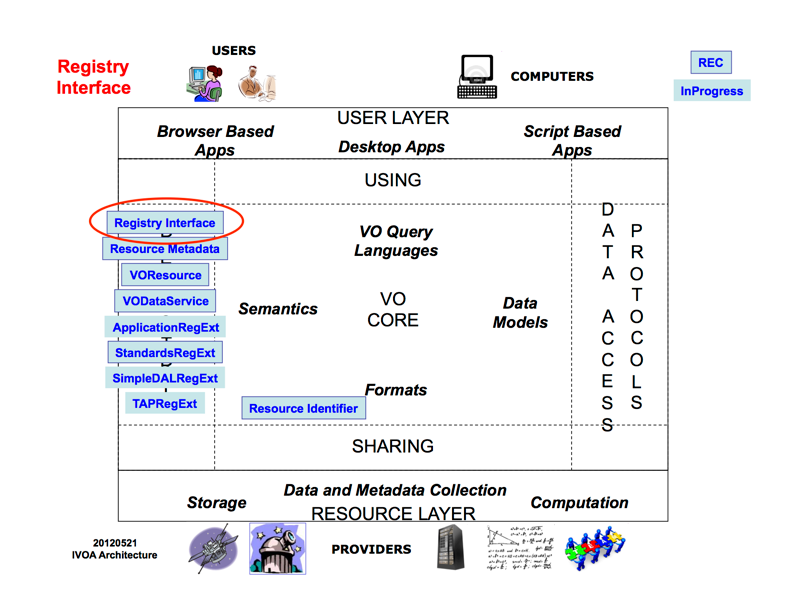
\includegraphics[width=0.9\textwidth]{archdiag.png}
\caption{IVOA Architecture
diagram with the Registry Interface specification (RI) and
the related standards marked up.}
\label{fig:arch}
\end{center}
\end{figure}

This specification directly relates to other VO standards in the
following ways:


\begin{bigdescription}
\item[VOResource \citep{std:VOR}]VOResource sets the foundation for a
formal definition of the data model for resource records via its schema
definition.

\item[IVOA Identifiers \citep{std:VOID2}]IVOA identifiers are something like
the primary keys to the VO registry.  Also, the notion of an authority as
laid down in IVOA Identifiers plays an important role as publishing
registries can be viewed as a realization of a set of authorities.

\end{bigdescription}


\section{The IVOA Harvesting Interface}

\label{harvesting}

The harvesting interface allows the retrieval of complete VOResource
records from registries supporting harvesting.  Publishing registries
MUST support the IVOA harvesting interface, searchable registries SHOULD
do so.

The IVOA harvesting interface is built on the standard Protocol for
Metadata Harvesting developed by the Open Archives Initiative, OAI-PMH
\citep{std:OAIPMH}.  In this section, after giving a brief introduction
to OAI-PMH, we define additional constraints and requirements for
OAI-PMH services to be interoperable with the VO environment.

In version 1.0 of this document, a variant of the OAI-PMH
protocol was defined using SOAP in the exchange of messages.  Version
1.1 no longer defines it (although of course there is no requirement to
remove it from running services); since OAI-PMH over SOAP has never been
in active use by the IVOA, we consider this still a minor specification
change not warranting a new major version.

\subsection{The OAI Protocol for Metadata Harvesting}

\label{oaipmh}

While for details of OAI-PMH we refer to \citet{std:OAIPMH}, 
in the following we give a
brief overview of OAI-PMH that should be sufficient to understand the
protocol's role within the Registry interface architecture.

The OAI-PMH v2.0 specification defines:


\begin{itemize}

\item the meaning and behavior of the six harvesting operations, referred
to as verbs,{}

\item the meaning of the input arguments for each operation, and{}

\item the XML Schema used to encode response messages.{}
\end{itemize}

The six standard operations laid down in OAI-PMH are:


\begin{bigdescription}
\item[Identify] provides a description of the registry

\item[ListIdentifiers]returns a list of identifiers for the resource
records held by the registry, possibly restricted to records changed
within a certain time span or to those belonging to a certain set.

\item[ListRecords]returns complete resource records in the registry,
possibly restricted to records changed within a certain time span or to
those belonging to a certain set.

\item[GetRecord]returns a single resource description matching a given
identifier.

\item[ListMetadataFormats]returns a list of supported formats that the
registry can use to encode resource descriptions upon a harvester's
request.

\item[ListSets]returns a list of set names supported by the registry
that harvesters can request in order to get back a subset of the
descriptions held by the registry.

\end{bigdescription}

The ListRecords and GetRecord operations return the actual resource
description records held by the registry. These descriptions are encoded
in XML and wrapped in a general-purpose envelope defined by the OAI-PMH
XML Schema (with the namespace
\texttt{http://www.openarchives.org/OAI/2.0}).

Through the operations' arguments, OAI-PMH provides a number of useful
features:


\begin{itemize}

\item Support for multiple return formats. As suggested by the existence
of the
\oaiop{ListMetadataFormats}  operation, a harvester can request the
formats available for encoding returned resource descriptions.{}

\item Harvesting by date. The \oaiop{ListIdentifiers}  and
\oaiop{ListRecords}  operations both support \texttt{from}  and
\texttt{until}  date arguments which restrict the response to records
changed withing the given, possibly half-open, interval.{}

\item Harvesting by category. The \oaiop{ListIdentifiers}  and
\oaiop{ListRecords} operations both support a set argument for
retrieving resources that are grouped in a particular category. Resource
records may belong to multiple sets.{}

\item Marking records as deleted. Registries may mark records as deleted
so that harvesters will be notified that a resource has become
unavailable even if only performing incremental harvests.

\item Support for resumption tokens. If a request results in returning a
very large number of records, the registry can choose to split the
results over several calls; this is done by passing a resumption token
back to the harvester. The harvester uses it to retrieve the next set of
matching results.{}

\end{itemize}
It is important to note that the OAI-PMH interface is not intended
to be a general search interface. The filtering capabilities described
above are just enough to support intelligent harvesting between
registries. Most end-user applications will use a dedicated search
interface on a searchable registry (cf.~sect.~\ref{sect:searching}).

In addition to basic OAI-PMH compliance, this specification defines
a set of OAI-PMH-compliant requirements and recommendations
special to OAI-PMH's use within the VO that are described in the
remaining subsections.


\subsection{Metadata Formats for Resource Descriptions}

\label{sect:metadataformats}

All IVOA registries that support the Harvesting Interface must support
two standard metadata formats: the OAI Dublin Core format (mandated by
the base OAI-PMH standard) and the IVOA VOResource metadata format
\citep{std:VOR}.

The VOResource metadata format has the metadata prefix name
\texttt{ivo\_vor}, which can be used wherever \citet{std:OAIPMH} allows a
metadata prefix name.  The format uses the VOResource core XML Schema
with the namespace 
\texttt{http://www.ivoa.net/xml/VOResource/v1.0}
(recommended namespace prefix \xmlel{vr:}) along with any legal
extension of this schema to encode the resource descriptions within the
OAI-PMH metadata tag from the OAI XML Schema (namespace
\texttt{http://www.openarchives.org/OAI/2.0}, recommended namespace
prefix \xmlel{oai:}). 

As VOResource and its extensions do not define global elements, the
child element within \xmlel{oai:metadata} needs to be separately
defined.  This specification does this by providing the
\xmlel{ri:Resource} element.  It is defined in a schema with the target
namespace
\nolinkurl{http://www.ivoa.net/xml/RegistryInterface/v1.0}, which is given
in appendix~\ref{app:rischema}.

The
\xmlel{ri:Resource} element MUST include an \xmlel{xsi:type} attribute
that assigns the element's type to \xmlel{vr:Resource} or one of its
legal extensions.

It is strongly recommended that all QName values of \xmlel{xsi:type}
attributes within the VOResource record use XML namespace prefixes as
recommended in VOResource or the VOResource extensions.  Minor version
changes are not in general reflected in the recommended prefixes --
e.g., both VODataService 1.0 and VODataService 1.1 use \xmlel{vs:}.
Registry operators
who must deliver OAI-PMH documents containing resource records written
to different versions of a registry extension are advised to
override the prefix
bindings on the element level if at all possible.

The OAI Dublin Core format, with the metadata prefix of \texttt{oai\_dc},
is defined by the OAI-PMH base standard and must be supported by all
OAI-PMH compliant registries.

Harvestable registries may support other metadata formats. Responses to
the
\oaiop{ListMeta\-dataFormats} operation 
must list all names for formats supported
by the registry; even though they are mandatory, this list must include
\texttt{ivo\_vor} and \texttt{oai\_dc}.


\subsection{Identifiers in OAI Messages}

\label{oaiidentifiers}

In accordance with the OAI-PMH standard, an OAI-PMH XML envelope that
contains a resource description must include a globally unique URI that
identifies that resource record. This identifier must be the IVOA
identifier used to identify the resource being described as given in
its \xmlel{vr:identifier} child element.

This specification does not follow the recommendation of the OAI-PMH
standard with regard to record identifiers. OAI-PMH makes a distinction
between the resource record containing resource metadata and the
resource itself; thus, it recommends that the identifier in the OAI
envelope be different from the resource identifier. In particular, the
former is the choice of the publishing registry. This allows one to
distinguish resource descriptions of the same resource from different
registries, which in principle could be different.

In the VO, because it is intended that resource descriptions of the
same resource from different registries should not differ (apart from
possible additions of \xmlel{vr:validationLevel} elements), there
is not a strong need to distinguish between the resource and the
resource description. 

By making the resource and resource record
identifiers the same, it becomes much easier to retrieve the record for
a single resource via \oaiop{GetRecord}, regardless of which
registry is being queried.  Otherwise -- when the registry chooses
the record identifier -- a client will not a priori know the record
identifier for a particular resource, and so it is left to call
\oaiop{ListRecords}  and search through the metadata of all the
records itself to find the one of interest. In contrast, IVOA
identifiers are intended to be a cross-application way of referring to a
resource, and thus when a client wants only a single specific resource
record, it is very likely that it would know the resource identifier
when making a call to the \oaiop{GetRecord} operation.


\subsection{Required Records}
\label{oairequired}

This section describes the records that a harvestable VO registry
must include among those it emits via the OAI-PMH operations.

The harvestable registry MUST return one record that describes the
registry itself as a whole, and the \texttt{ivo\_vor}  format MUST be
supported for this record. This record is also included in the
\oaiop{Identify} operation response.  When encoded using the
\texttt{ivo\_vor} format, the returned \xmlel{ri:Resource} element must
be of the type \xmlel{vg:Registry} from the VORegistry schema
(see sect.~\ref{sect:vgharvest}). The
record MUST include a \xmlel{vg:managedAuthority} for every authority
identifier that originates at that registry.

Additions to the list of a registry's managed authorities must follow
the protocol outlined in sect.~\ref{sect:authres}.

The harvestable registry must be able to return exactly one record in
\texttt{ivo\_vor}  for each authority identifier listed as a
\xmlel{vg:managedAuthority} in the \xmlel{vg:Registry} record
that describes that registry. When encoded in the \texttt{ivo\_vor}
format, the type of these elements must be \xmlel{vg:Authority}.


\subsection{The Identify Operation}

\label{sect:oaiidentify}

The \oaiop{Identify}  operation describes the harvestable registry as a
whole.  The response from this operation must include all information
required by the OAI-PMH standard. In particular, it must include an
\xmlel{oai:baseURL} element that must refer to the base URL to the
harvesting interface endpoint.  The \oaiop{Identify}  response must
include an \xmlel{oai:description} element containing a single
\xmlel{ri:Resource} element with an \xmlel{xsi:type} attribute that
sets the element's type to \xmlel{vg:Registry}. The content of
\xmlel{vg:Registry} type must be the registry description of the
harvestable registry itself.

In its \oaiop{Identify} response, an OAI-PMH-compliant registry must
declare its support for deleted records.  This can be one of

\begin{description}

\item[\texttt{no}] -- the registry will never notify harvesters of
records that have become unavailable.  In an enviroment like the VO, 
where searchable registries frequently harvest publishing registries,
this is severely discouraged, as without deleted records, harvesters
need to perform full harvests every time or risk delivering stale
records.
\item[\texttt{transient}] -- the registry will notify harvesters of
records that have become unavailable, but the deleted records will
entirely vanish after some time.  This specification adds to the OAI-PMH
requirements that registries declaring \texttt{transient} support MUST
keep their deleted records for at least six months (after which they may
discard them).
\item[\texttt{persistent}] -- the registry promises to indefinitely keep
deleted records.
\end{description}

\subsection{IVOA Supported Sets}

\label{supportedsets}

Sets, as defined in the OAI-PMH standard, are ``an optional construct
for grouping items for the purpose of selective harvesting'' (see 
\citet{std:OAIPMH}, section 2.6). Harvestable IVOA registries are free
to define any number of custom sets for categorizing records. The
OAI-PMH standard allows a record to be a member of multiple sets.

This specification defines one reserved set name with a special
meaning; future versions of this specification may define additional set
names.  These reserved set names will all start with the characters
\texttt{ivo\_}; implementors should not define their own set names
that begin with this string. While support for sets is optional 
in the OAI-PMH standard, a VO registry MUST support
the set with the reserved name \texttt{ivo\_managed} to be compliant
with this specification.

The \texttt{ivo\_managed} set refers to all records that originate from the
queried registry. That is, those records that were harvested from other
registries are excluded. The resource identifiers given in the
records MUST have an authority identifier that matches on one of the
\xmlel{vg:managedAuthority} values in the \xmlel{vg:Registry}
record for that registry.  Full searchable registries may use this set
while harvesting other registries to avoid getting duplicate records.

\subsection{Time Granularity}

\label{sect:timegranularity}

Datestamps in the OAI-PMH 2.0 standard are encoded using ISO8601 and
expressed in UTC, with the UTC designator ``Z'' appended to seconds-based
granularity where supplied, i.e. \texttt{YYYY-MM-DDThh:mm:ssZ}. In
general OAI-PMH registries, granularity at seconds scale is optional.
Harvestable IVOA registries MUST report datestamps at the granularity of
seconds and accept \texttt{from} and \texttt{until} arguments in the same format. This
simplifies the incremental harvesting process in the multi-registry IVOA
environment.

\section{Registering Registries}
\label{regreg}

Harvesting registries must able to locate remote registry resources
relevant to them, and both harvesting registries and clients need access
to metadata for the registry service itself. We address both of these
issues by providing a schema for describing registries themselves, and a
repository for indexing them.

The resource specification for registries themselves is defined by an
\xmlel{ri:Re\-source} extension \xmlel{vg:Registry}, which describes 
metadata of the registry itself and its support for interfaces 
described in this document or elsewhere. 
These resources are themselves stored as
records in registries as described in \ref{oairequired}. From each
identifier, further IVOA identifiers for authority information,
services, and other records belonging under that publishing umbrella 
may be created. A publishing registry is said to exclusively manage a 
naming authority on behalf of the owning publisher; this means that 
within the IVOA registry network, only that specific registry may 
publish records having identifiers which begin with that authority identifier.

The XML namespace URI of this schema is
\nolinkurl{http://www.ivoa.net/xml/VORegistry/v1.0}.  It has been chosen
to allow it to be resolved as a URL to the XML Schema document, which is
also given in appendix~\ref{app:vgschema}. The recommended prefix for
this namespace is \xmlel{vg:}.

The schema has not been changed from the one used in version 1.0,
although the standard contents have somewhat changed.  The rationale for
keeping the schema unchanged is that the presence of schema features no longer relevant
has no detrimental consequences for Registry operations, whereas changing
the schema could break already operational clients.


\begin{figure}[th]
\begin{lstlisting}[language=XML]
<ri:Resource status="active" xsi:type="vg:Authority" 
   updated="2006-07-01T09:00:00" created="2006-07-01T09:00:00">
  <title>IVOA Naming Authority</title>
  <shortName>IVOA</shortName>
  <identifier>ivo://ivoa.net</identifier>
  <curation>
    <publisher ivo-id="ivo://ivoa.net/IVOA">International Virtual 
      Observatory Alliance</publisher>
    <creator>
      <name>Raymond Plante</name>
      <logo>http://www.ivoa.net/icons/ivoa_logo_small.jpg</logo>
    </creator>
    <date>2006-07-01</date>
    <contact>
      <name>IVOA Resource Registry Working Group</name>
      <email>registry@ivoa.net</email>
     </contact>
  </curation>
  <content>
    <subject>virtual observatory</subject>
    <description>This registers the IVOA as the owner of the ivoa.net
      authority identifier.</description>
    <referenceURL>http://rofr.ivoa.net</referenceURL>
  </content>
  <managingOrg>International Virtual Observatory Alliance</managingOrg>
</ri:Resource>
\end{lstlisting}

\caption{A sample \xmlel{vg:Authority}-typed resource record as it would
be delivered within \xmlel{oai:metadata}.  XML namespace declarations 
for the prefixes \xmlel{ri:}, \xmlel{xsi:}, and \xmlel{vg:} are
assumed on enclosing elements.}
\label{fig:authrecord}
\end{figure}

\subsection{The Authority Resource Extension and the Publishing Process}

\label{sect:authres}


The \xmlel{vg:Authority} type extends the core \xmlel{vr:Resource}
type to specifically describe the ownership of an authority identifier
by a publishing organization.

The IVOA identifier of a \xmlel{vg:Authority} record provided via the
\xmlel{vr:identi\-fi\-er} element must have an empty resource key component
as defined in \citet{std:VOID}.

The meaning of a \xmlel{vg:Authority} record is that the organization
referenced in the \xmlel{vg:managingOrg} element has the sole right to
create (in collaboration with a publishing registry) and register
resource descriptions using the authority identifier given by the
\xmlel{vr:identifier} element.

Before a publisher can create resource descriptions using a new
authority identifier, it must first register its claim to the authority
identifier by creating a \xmlel{vg:Authority} record.  Before the
publishing registry commits the record for export, it must first search
a full registry to determine if a \xmlel{vg:Authority} with this
identifier already exists; if it does, the publication of the new
\xmlel{vg:Authority} record must fail. 

When a registry creates a
\xmlel{vg:Authority} record, it is said that the registry manages the
associated authority identifier (on behalf of the owning publisher)
because only that registry may create records with identifiers beginning
with that authority identifier. The registry must also document this ownership
by adding a corresponding \xmlel{vg:managedAuthority} element to the 
registry's own resource record.

The mechanism outlined here is not free of potential conflicts in the distributed
environment of the VO Registry.  The IVOA Registry Working group
periodically monitors the registry-authority graph to ensure each
authority in the Registry is claimed by exactly one registry.

\subsection{Describing Registries with the Registry Resource Extension}

\label{sect:resext}

The \xmlel{vg:Registry} type extends the core \xmlel{vr:Service} type to
specifically describe registries in order to support discovering them
and collecting their metadata; in addition, the extension type also
defines the VO-specific metadata in the response to an OAI-PMH
\oaiop{Identify} request.  

As a subclass of \xmlel{vr:Service}, the \xmlel{vg:Registry}
type uses \xmlel{vr:capability} elements to describe its support for
network interfaces to the services.  The specific types defined here
derive from an intermediate restriction on \xmlel{vr:Capability} called
\xmlel{vg:RegCapRestriction} to force the value of the
\xmlel{standardID} attribute to be \nolinkurl{ivo://ivoa.net/std/Registry}.
In particular, OAI-PMH endpoints as specified here are identified by
\nolinkurl{ivo://ivoa.net/std/Registry}.  Client should discover
registries by looking for records with capabilities declaring
this \xmlel{standardID}.

If the \xmlel{vg:full} element in an \xmlel{vg:Registry} instance
is set to \texttt{true}, it indicates the registry's intent to
accept all valid resource records it harvests from other
registries in accordance with the OAI-PMH specification.  This will
typically be searchable registries implementing some Registry search
interface, but there are also use cases for full registries only
implementing OAI-PMH (and thus only providing an \xmlel{vg:Harvest} 
capability).

The \xmlel{vg:managedAuthority} is used by publishing registries  to
claim an authority identifier (see also sect.~\ref{oairequired}).  Note
that for each managed authority claimed, the registry MUST provide a
\xmlel{vg:Authority}-typed resource record for that authority identifier
within its \texttt{ivo\_managed} set.

As of version 1.1 of this specification, VO registry records must provide
the three mandatory VOSI capabilities: availability, a listing of
service capabilities, and a listing of tables if relevant, i.e. if a
RegTAP or other tabular interface is available \citep{std:VOSI}.


\subsection{The Search Capability}
\label{sect:vgsearch}

Version 1.0 of this standard defined a search interface, and such
interfaces are described by capabilites of the type \xmlel{vg:Search}.
Since in this version, search interfaces are specified by external
standards, such external standards may define differing ways of
discovering them\footnote{For instance, RegTAP \citep{std:RegTAP} uses
the \xmlel{tre:dataModel} element from TAPRegExt as its primary
discovery mechanism in its version 1.0.}.  The search capability nevertheless is 
not removed from the schema for backward compatibility, and is available in appendix
\ref{app:RISearch}.

\subsection{The Harvesting Capability}

\label{sect:vgharvest}

A registry declares itself to be a harvestable registry by including a
\xmlel{vr:capabi\-li\-ty} element with an \xmlel{xsi:type} 
attribute set to \xmlel{vg:Harvest}. An example capability for this
type is provided in the appendix \ref{sect:exampleCap}.

A \xmlel{vr:capability} element of type \xmlel{vg:Harvest} MUST
include at least one \xmlel{vr:interface} element with an
\xmlel{xsi:type} attribute set to \xmlel{vg:OAIHTTP} and the
\xmlel{role} attribute set to \texttt{std}. If the
\xmlel{vr:capability} element is used to simultaneously describe
support for other versions of this Registry Interface standard, then the
\xmlel{vr:interface} element describing support for this version must
include the version attribute set to \texttt{1.0}. The
\xmlel{vr:accessURL} element must be set to the base URL for the
OAI-PMH interface.

The \xmlel{vg:OAISOAP} extension of \xmlel{vr:WebService}
was defined in version 1.0 of this specification and is no longer part of VO
Registry interfaces since it was never used.

\section{Registry Discovery}

\subsection{The Registry of Registries}

\label{sect:rofr}

To facilitate discovery and automated harvesting of VO publishing registries,
a master list of IVOA registries exists as part of the IVOA web 
infrastructure, hosted at \nolinkurl{http://rofr.ivoa.net}. 
It is referred to as the Registry of Registries, or RofR (pronounced ``rover''). 
As the RofR is itself a registry, it provides an OAI-PMH interface conforming 
to this document. The OAI-PMH interface is always available at
\nolinkurl{http://rofr.ivoa.net/oai}. The RofR includes resource records 
describing each currently active registry of IVOA resources, its status
as a full or local registry, authorities associated with it, and its 
programmatic interfaces. Each record is of type \xmlel{vg:Registry} as 
defined in section \ref{sect:resext}. 

Once a registry provider has deployed a new publishing registry, they
must enroll it the RofR for their records to be seen by the full 
searchable registries, and therefore registry search clients accessing 
the whole IVOA registry ecosystem. The RofR provides a dedicated 
web-based interface for this purpose accessible
from \nolinkurl{http://rofr.ivoa.net}.  The RofR includes a
validator package, which thoroughly checks the new registry, including
schema validation for the OAI interface itself and all listed resources.
The registration process will only accept registries that validate
successfully.  Local updates within a publishing registry post-inclusion
in the RofR are not necessarily automatically validated by the RofR
software later: the validator tool can, and indeed should, be used
independently of the initial admission process by the registry providers
to periodically make sure their registries are still compliant with the
relevant IVOA standards. 

The Registry of Registries also contains resources describing
the most recent versions of IVOA standards for resources and
resource extensions themselves; these are of type \xmlel{vstd:Standard}. 
It is not guaranteed that every standard will be represented in RofR,
but for the ones that are listed, the RofR version of their document
is the canonical version.

\subsection{Harvesting the Registry of Registries}

\label{sect:harvestrofr}

Given the Registry of Registries contains records for all other
currently active and validated IVOA registries, a client wishing to
harvest the contents of all registries should begin at the RofR. Full 
searchable registries wishing to include records from the other IVOA
registries count among these potential clients. To harvest the entire
contents of IVOA registries, it is recommended to first harvest the
Registry of Registries via its OAI-PMH interface.

This first step is done by making a call to the RofR's OAI-PMH interface
with the \textbf{ListRecords} operation, with the \textbf{set} argument
set to \textbf{ivo\_publishers}. This will return the registry records
(i.e. resources with xsi:type='vg:Registry') for the registries that
successfully registered themselves as described in \ref{sect:rofr}. 

The next step in harvesting the entire distributed IVOA registry
contents is to iterate over the \xmlel{accessURL} of each
\xmlel{vg:Registry} record's \xmlel{vr:capability} of type
\xmlel{vg:Harvest}, and use the URL for each of those OAI-PMH interfaces
to harvest the individual registries. In iterating over the OAI interface
of each registry itself, to avoid harvesting duplicate records from the 
full searchable registries, it is recommended to add the \texttt{set} 
parameter to that OAI query as well: records locally published by 
a full registry comprise that registry's supported set \texttt{ivo\_managed}.

The very first time the harvester executes the \textbf{ListRecords}
operation on the RofR or any listed registry, the \textbf{from} argument
should be not used so that all known publishing registries are returned,
as well as all known resources within each discovered registry. If the
harvesting client wishes to use the OAI interface for incremental
updates, it can cache at least a mapping of the registry identifiers to
their respective harvesting endpoints along with a timestamp for when
this operation was last successfully carried out on each. Then, at the
start of subsequent harvesting updates, the harvester can provide the
cached date using the \textbf{from} argument to receive only new and
updated records, and update the cached timestamp upon success.  

Experience has shown that when relying on incremental harvests
exclusively, minor problems eventually accumulate to severe
inconsistencies even when registries declare support for deleted
records.  It is therefore recommended that harvesting clients occasionally
(e.g., semianually) perform full updates to an empty local copy without 
using the \textbf{from} parameter, even for registries that announce
deletion of records. To further provide some robustness against small
operational issues in the publishing process, it is also recommended 
to leave an overlap in incremental harvesting requests, e.g. to request 
resources going back to the beginning of the day of last incremental harvest.


For example, to get a listing of registries in the IVOA ecosystem, one
would first query
\begin{verbatim}
http://rofr.ivoa.net/oai?verb=ListRecords
                        &metadataPrefix=ivo_vor
                        &set=ivo_publishers.
\end{verbatim}


Then, for each returned resource, the \xmlel{accessURL} under a
\xmlel{Capability} with \xmlel{xsi:type=vg:Harvest}, that URL could be
called as such:

\begin{verbatim}
http://accessURLValue?verb=ListRecords&metadataPrefix=ivo_vor
\end{verbatim}
or
\begin{verbatim}
http://accessURLValue?verb=ListRecords
                     &metadataPrefix=ivo_vor
                     &from=YYYY-MM-DDTHH:MM:SSZ
\end{verbatim}
for return visits, with the 'from' date representing the last successful
query to that accessURL. 

\section{Searching Registries}
\label{sect:searching}

Experience with version~1 of this specification suggests that it is
preferable to not couple the relatively stable standards for harvesting and
general registry maintenance with client interfaces to the registry,
which were found to be in much more need of experimentation.  For a
discussion of the history of client interfaces in the VO, see
\citet{paper:regclient}.

\subsection{RI Search}
\label{RISearch}
A SOAP-based search capability, \xmlel{vg:RISearch} defined in Registry 
Interfaces 1.0, exists but is no longer encouraged or required for searchable
registries as technologies have moved forward. However, it is still a valid
capability defined in the registry resource schema so that registry  operators 
may continue to provide valid RI1 registries without having to support different 
versions of the VORegistry schema. The base \xmlel{vg:RISearch} extension may 
also be useful for the description of future registry search interfaces. RISearch 
is described in appendix~\ref{app:RISearch}.


\subsection{Registry Table Access Protocol Services}
\label{RegTAP}

One second-generation standard search interface to the VO Registry that
has progressed to become an IVOA recommendation is RegTAP
\citep{std:RegTAP}, an interface based on a relational representation of
key fields in resourcce descriptions and on the IVOA Table Access Protocol 
\citep{std:TAP}. RegTAP services have been made available from several 
registry providers listed in the Registry of Registries.

RegTAP-based registries should be located by clients as described 
in the RegTAP standard (which in version 1.0 happens through locating 
TAP services with a certain data model identifier like 
\nolinkurl{ivo://ivoa.net/std/RegTAP#1.0}).  To aid smart clients of
the full RofR which generate lists for initial discovery, RegTAP registries 
must also be registered as separate resources with the appropriate tableset.  
These must include either a full TAP service capability according to
TAPRegExt \citep{std:TAPREGEXT-20120827} or an auxiliary capability
referencing a TAP service as per \citet{note:DataCollect}.  An example
for the latter option, preferable if the TAP service in question
contains additional tables, is given in appendix \ref{sect:exampleCap}.

\subsection{Announcing Local vs Full Searchable Registries}
\label{FullSearch}

While a publishing registry may provide search capabilities for its
own hosted records, this is considered a locally searchable registry,
and not a full searchable one, as distinguished in the RofR listing. 
For a registry to be considered full searchable, it must harvest resources 
from the other publishing  registries listed in the RofR, and implement 
an IVOA standard programmatic interface beyond the interface for OAI harvesting,
with some method for filtering resource queries. 
This can be announced simply in the registry's own self-describing resource
record with a \xmlel{full} tag set to true, without having to proscribe any 
one interface as the defining search feature.

\section{Looking Forward}
\label{LookingForward}

While the OAI-PMH harvesting interface as adopted from outside the IVOA 
community is stable and replacing it would require a major revision
of this document, we expect that new search interfaces for registries will
be continually developed, leveraging new technologies and best practices
as they emerge. These search interfaces can be added without sacrificing 
interoperability with the IVOA registry ecosystem.  Whether these emerging 
search technologies become formally endorsed by the IVOA as notes or new 
standards documents, so long as a registry supports the basic harvest interface 
and hosts valid \xmlel{ri:Resource} documents including registry and authority 
records, it should be considered covered by the practices described herein and 
a welcome addition to the Registry of Registries listing, with all of its 
records also accessible through the full registries.

\appendix

\section{The RegistryInterface Schema}
\label{app:rischema}

The following schema defines a global element, allowing the inclusion of
VOResource records into \xmlel{oai:metadata} elements in OAI-PMH
responses for the \texttt{ivo\_vor} metadata prefix.  See 
sect.~\ref{sect:metadataformats} for details.

The schema is unchanged from version 1.0 of this specification and
therefore does not change its version.

\lstinputlisting[language=XML,basicstyle=\footnotesize]{RegistryInterface-1.0.xsd}

\section{The VORegistry Schema}
\label{app:vgschema}

The following schema defines VOResource types for describing registries
in the Registry.  It is unchanged from version 1.0 of this specification
and therefore does not change its version.

Note that standards defining search interfaces may specify alternative
or complementary methods of registering the services defined by them,
and that auxiliary capabilities for these search capabilities may be
listed within the registry record.

\lstinputlisting[language=XML,basicstyle=\footnotesize]{VORegistry-1.0.xsd}

\section{Example Capabilities}
\label{sect:exampleCap}

The following XML fragment shows the three capability elements discussed
in this document: The OAI-PMH-based publishing registry, the legacy 
RI 1.1 searchable registry, and an auxiliary TAP capability as used
for RegTAP.

\begin{lstlisting}[language=XML,basicstyle=\footnotesize]
<ri:Resource
  xmlns:vg="http://www.ivoa.net/xml/VORegistry/v1.0" 
  xmlns:xsi="http://www.w3.org/2001/XMLSchema-instance"
  xmlns:xmlns:ri="http://www.ivoa.net/xml/RegistryInterface/v1.0">

  <!-- Standard VOResource metadata omitted for brevity -->

  <!-- The capability for an OAI-PMH endpoint (publishing registry) -->
  <capability xsi:type="vg:Harvest" standardID="ivo://ivoa.net/std/Registry">
    <interface xsi:type="vg:OAIHTTP" version="1.0" role="std">
       <accessURL use="base">http://registry.example.org/oai</accessURL>
    </interface>
    <maxRecords>100</maxRecords>
  </capability>

  <!-- A legacy, RI1.0 searchable registry endpoint, with an
    extra interface for web browsers. -->
  <capability xsi:type="vg:Search" standardID="ivo://ivoa.net/std/Registry">
    <interface xsi:type="vr:WebBrowser" version="1.0" role="gui">
      <accessURL use="full">http://registry.euro-vo.org</accessURL>
    </interface>
    <interface xsi:type="vr:WebService" version="1.0" role="std">
      <accessURL use="full"
        >http://registry.example.org/services/RegistrySearch</accessURL>
    </interface>
    <maxRecords>100</maxRecords>
      <extensionSearchSupport>core</extensionSearchSupport>
  </capability>

  <!-- A reference to RegTAP-enabled TAP service as an auxiliary
    capability -->
  <capability standardID="ivo://ivoa.net/std/TAP#aux">
    <interface xsi:type="vs:ParamHTTP" role="std">
      <accessURL use="base">http://registry.example.org/tap</accessURL>
    </interface>
  </capability>

   <!-- A RegTAP-capable searchable registry should have a tableset
   with all its tables in the rr schema here -->
</ri:Resource>
\end{lstlisting}

\section{The RISearch Schema}
\label{app:RISearch}

The following schema defines the SOAP-based RISearch interface, which
is discouraged as of version 1.1 but still available. 
It is unchanged from version 1.0 of this specification
and therefore does not change its version.

% GENERATED: !schemadoc VORegistry-1.0.xsd Search
\begin{generated}
\begingroup
      	\renewcommand*\descriptionlabel[1]{%
      	\hbox to 5.5em{\emph{#1}\hfil}}\vspace{2ex}\noindent\textbf{\xmlel{vg:Search} Type Schema Documentation}

\noindent{\small
            The capabilities of the Registry Search implementation.  
         \par}

\vspace{1ex}\noindent\textbf{\xmlel{vg:Search} Type Schema Definition}

\begin{lstlisting}[language=XML,basicstyle=\footnotesize]
<xs:complexType name="Search" >
  <xs:complexContent >
    <xs:extension base="vr:Capability" >
      <xs:sequence >
        <xs:element name="maxRecords" type="xs:int" />
        <xs:element name="extensionSearchSupport"
                  type="vg:ExtensionSearchSupport" />
        <xs:element name="optionalProtocol"
                  type="vg:OptionalProtocol"
                  minOccurs="0"
                  maxOccurs="unbounded" />
      </xs:sequence>
    </xs:extension>
  </xs:complexContent>
</xs:complexType>
\end{lstlisting}

\vspace{0.5ex}\noindent\textbf{\xmlel{vg:Search} Extension Metadata Elements}

\begingroup\small\begin{bigdescription}\item[Element \xmlel{maxRecords}]
\begin{description}
\item[Type] \xmlel{xs:int}
\item[Meaning] 
                        The largest number of records that the registry search
                        method will return.  A value of zero or less indicates
                        that there is no explicit limit.  
                     
\item[Occurrence] required

\end{description}
\item[Element \xmlel{extensionSearchSupport}]
\begin{description}
\item[Type] string
\item[Meaning] 
                     	(deprecated)
                     
\item[Occurrence] required

\item[Allowed Values]\hfil
\begin{longtermsdescription}
\item[core]
                 Only searches against the core VOResource metadata are 
                 supported.
              
\item[partial]
                 Searches against some VOResource extension metadata are 
                 supported but not necessarily all that exist in the registry.
              
\item[full]
                 Searches against all VOResource extension metadata contained 
                 in the registry are supported.
              
\end{longtermsdescription}
\item[Comment] 
                     	This was used in Registry Interfaces 1.0 to indicate
                     	what VOResource extensions a search interface supported.
                     	Modern search interfaces will indicate that through
                     	version, their tableset, or similar.
                     

\end{description}
\item[Element \xmlel{optionalProtocol}]
\begin{description}
\item[Type] string
\item[Meaning] 
                       (deprecated)
                     
\item[Occurrence] optional; multiple occurrences allowed.

\item[Allowed Values]\hfil
\begin{longtermsdescription}
\item[XQuery]
                 the XQuery (http://www.w3.org/TR/xquery/) protocol as defined
                 in the VO Registry Interface standard.  
              
\end{longtermsdescription}
\item[Comment] 
                       This was used in Registry Interfaces 1.0 to indicate
                       search protocol extensions.  In 1.1, use multiple
                       capabilities with the appropriate standardIDs
                       to declare special search capabilities.
                     

\end{description}


\end{bigdescription}\endgroup

\endgroup
\end{generated}

% /GENERATED


\section{Changes from Previous Versions}

\label{sect:changes}

For pre-REC-1.0 changes, see \citet{std:RI1}.

\subsection{Changes from first 1.1 WD}

\begin{itemize}

\item Text clarifications for harvesting the entire RofR, and 
exhortation to harvest from scratch occasionally as OAI 
announcement of record deletions are not mandatory.

\item Simplified announcement of full searchable registry
in the RofR and removed operational instructions which may change

\end{itemize}

\subsection{Changes from Version 1.0}

\label{changes-1.0}


\begin{itemize}

\item Corrected reference to OAI-PMH spec in registry interface
description to v2.0.

\item Added requirement for OAI-PMH interface to support seconds
granularity, optional in the OAI-PMH 2.0 standard itself. {}

\item Removed requirement for VOResource version number changes to force
an update of this document. {}

\item Removed the implementation-dependent requirement for searchable
registries in section 2, specifically the SOAP-based services
based on ``ADQL 1.0'' and XQuery.{}

\item Dropped the requirement on registries to not deliver any records
that are OAI-PMH deleted when no temporal constraint is given.{}

\item Added a requirement to provide VOSI endpoints.

\item Added support for auxiliary Registry TAP Service search interfaces

\item Clarified that the requirement to keep deleted records for six
months only applies to the transient case; also discouraging registries
with no support of deleted records.

\item Added recommended process for discovery of registries and their
resources using the Registry of Registries, based on the Registry of
Registries IVOA note

\item Added conclusion describing implications of future search and 
publishing interface changes in the Registry environment.

\item Many editorial changes across the text, mostly as a consequence of
externalizing search interfaces.

\end{itemize}


\bibliography{ivoatex/ivoabib,ivoatex/docrepo}

\end{document}
